\documentclass{beamer}
	% this is the preable
	%\usepackage[latin1]{inputenc}
	\usetheme{Copenhagen}
	%\usetheme{Berkeley}
	\title[Guessing missing enteries in a matrix]{Matrix completion}
	\author{Gursimran singh}
	\institute{Thapar university}
	\date{June 5,2012}

\begin{document}	
\begin{frame}
	\titlepage
\end{frame}

\begin{frame}{Singular value decmoposition}
	\begin{center}
		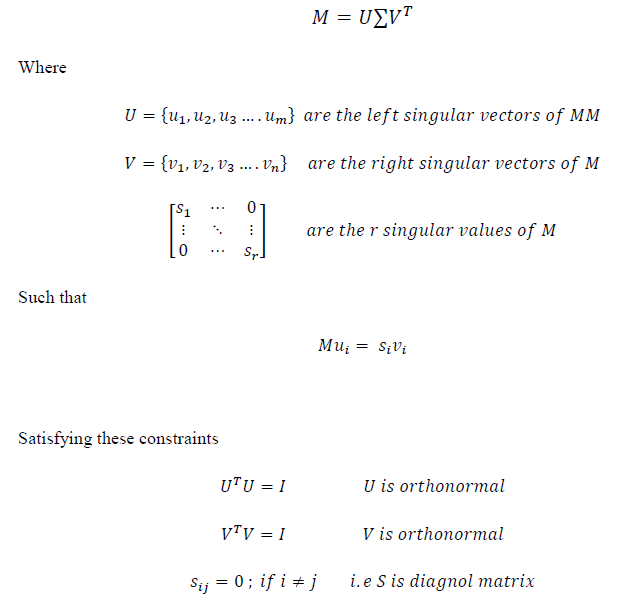
\includegraphics[scale=0.5]{myfig1.png}
	\end{center}
\end{frame}

\begin{frame}{Singular value decmoposition ... continued}
	\begin{center}
		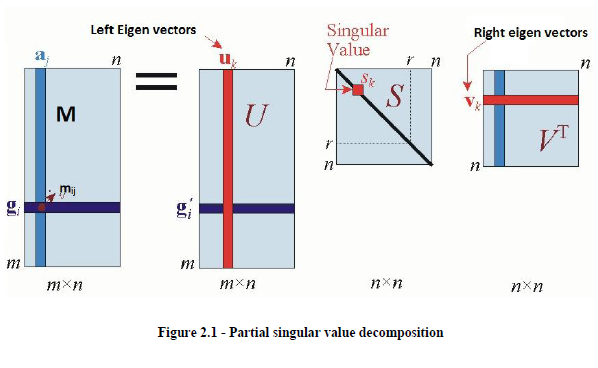
\includegraphics[ height = 80mm,width =105mm]{myfig2.png}
	\end{center}
\end{frame}

\begin{frame}{Principal Component Analysis}
	\begin{center}
		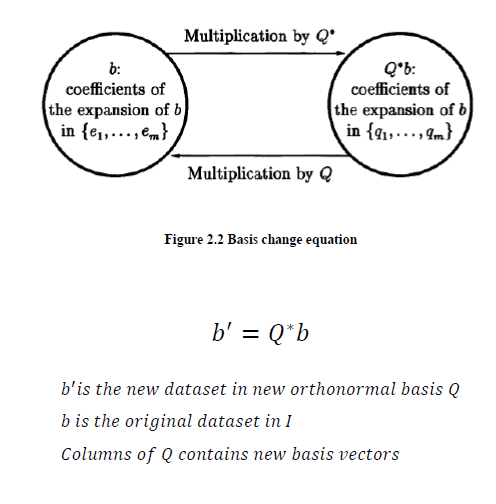
\includegraphics[ height = 70mm,width =80mm]{myfig3.png}
	\end{center}
\end{frame}

\begin{frame}{Principal Component Analysis}
	\begin{center}
		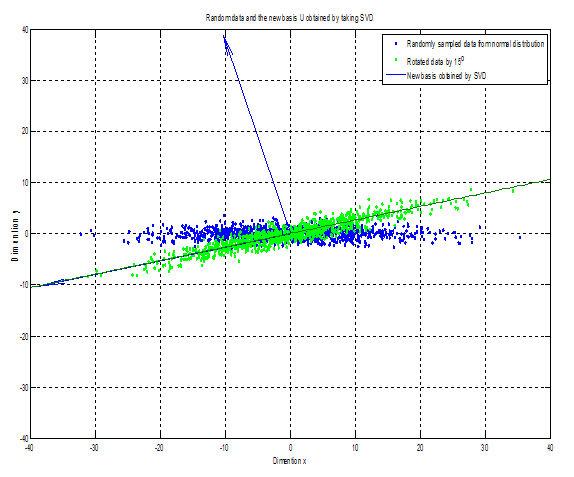
\includegraphics[ height = 70mm,width =80mm]{myfig4.png}
	\end{center}
\end{frame}

\begin{frame}{Principal Component Analysis}
	\begin{center}
		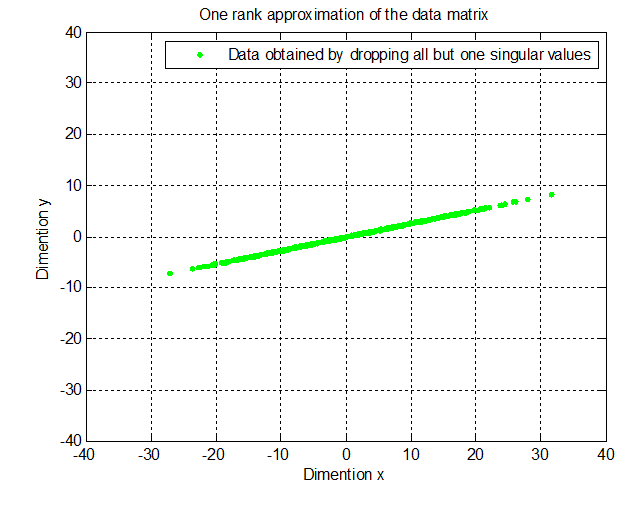
\includegraphics[ height = 70mm,width =80mm]{myfig5.png}
	\end{center}
\end{frame}

\begin{frame}{Matrix completion problem}
	\begin{center}
		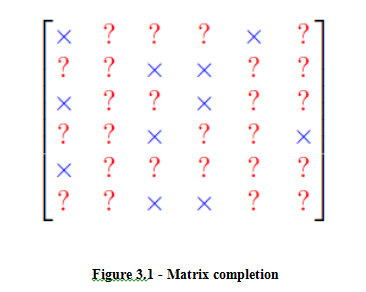
\includegraphics[ height = 70mm,width =80mm]{myfig6.png}
	\end{center}
\end{frame}



%\begin{frame}{How many degrees of freedom in a matirx?}
	% INCLUDE EARLIER WORK HERE...
%	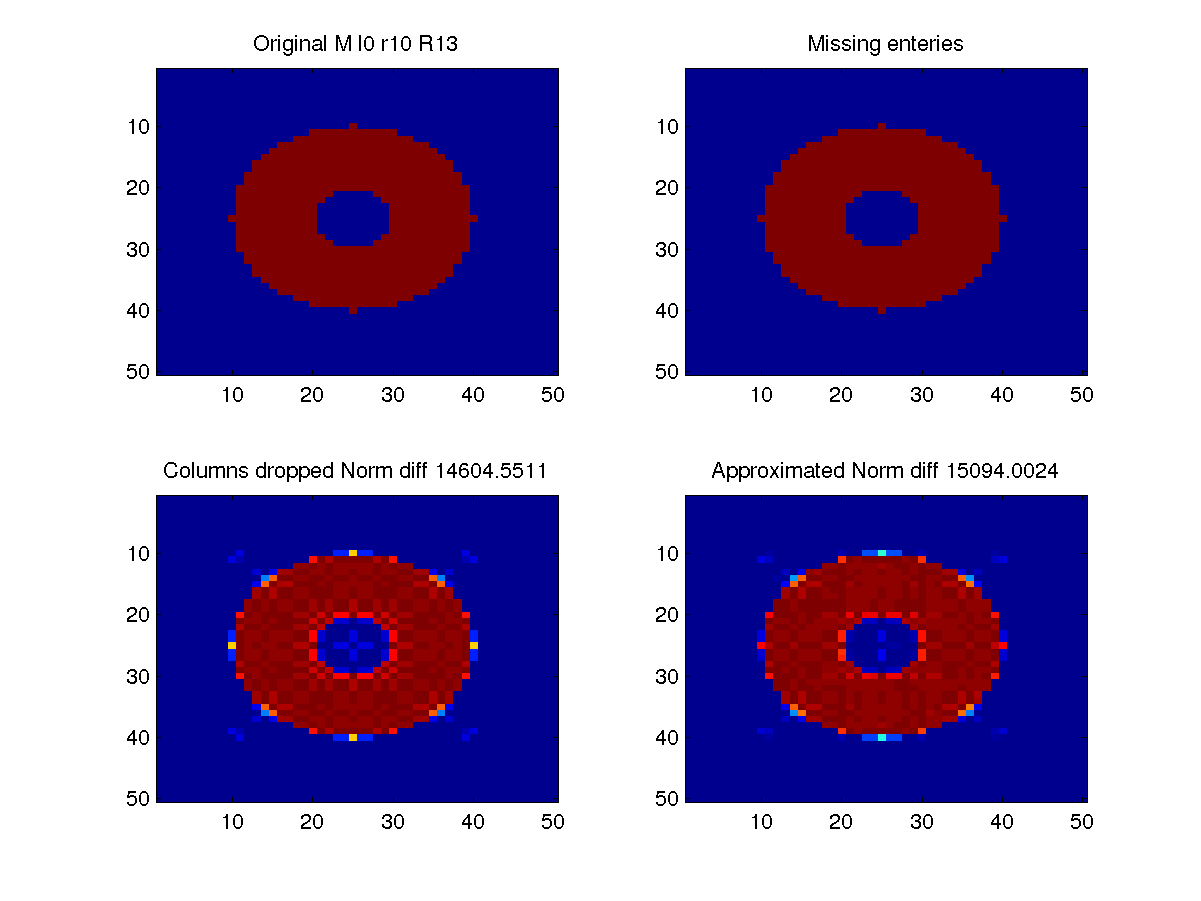
\includegraphics{hyperparabola.png}
%\end{frame}

\begin{frame}{Degrees of freedom in a matrix(n$\times$n) of rank r}

	$$ \textbf{r(2n-r)} $$
	\vspace {-5mm}
	\begin{block}{Proof of ${r(2n-r)}$}
		%\hspace{10mm}
		%\begin{center}
		$\Rightarrow nr +  (n-r)r$ \\
		$\Rightarrow nr + nr - r^2$  \\
		$\Rightarrow 2nr - r^2$  \\
		%\end{center}
	\end{block}
	
	\begin{itemize}
	  \item This will be of $\Theta$(nr) for a n$\times$n matrix of rank r.
	  \item which is much smaller than $\Theta$($n^2$).
	\end{itemize}
	\vspace{3mm}
	\begin{example}
	  For a matrix 1000x1000 of rank 20 we need just 40000 numbers instead of 1000000 numbers.
	\end{example}	
\end{frame}

\begin{frame}{Which set of $r(2n-r)$ numbers?}

	\textbf {Ofcourse not all sets of such numbers will work.}
	\begin{enumerate}
		\item If a complete row or column is missing, then you can't recover. There is no hope.
		\begin{item} If the matrix is something like this.
			$$M = e_1e_n^* = \left[
			\begin{array}{ccc}
			0&\cdots&1\\
			\vdots&\ddots&\vdots\\
			0&\cdots&0
			\end{array}
			\right]$$
		\end{item}

		\begin{item} or
			$$M = e_1x^* = \left[
			\begin{array}{ccc}
			x_1&\cdots&x_n\\
			0&0&0\\
			0&0&0
			\end{array}
			\right]$$
		\end{item}
		\vspace{3mm}
		\item So there are bunch of cases in which matrix recovery isn't going to work, whatsoever the method is..

	\end{enumerate}
	\vspace{5mm}
\end{frame}


\begin{frame}{Sample the matrix at random?}

	\begin{itemize}
		\item Only some combinitions of \textbf{$r(2n-r)$} numbers are going to be the right choice. (Good cases/ Bad cases)
		\begin{itemize}
			\item Matrix.
			\item No of enteries. ($>r(2n-r)$)
			\item Which combination of these enteries.
		\end{itemize}
		\vspace {3mm}
		\item What is \textbf{Probability} of exact matrix completion. Randomly sample
		\begin{enumerate}
			\item Matrix - Number of combinations of numbers that are GOOD cases.
			\item Number of samples ($>r(2n-r)$, otherwise its 0)
		\end{enumerate}
		%\item HOW? Sample the matrix Randomly choose atleast $r(2n-r)$ numbers from the matrix and see what happens for \textbf{most} of the cases.

	\end{itemize}

	\begin{block}{Central Idea!!}
		If I want the matrix to get completed for \textbf{most of cases (fixed probability)}, we will need \textbf{different amount of enteries ($>r(2n-r)$)} for different matrices. \\
		\center $Samlpes \propto \Psi_X(M)$ given some P
	\end{block}
\end{frame}

\begin{frame}{Coherence}
	$$ L \in R^{n \times n} = U \Sigma V^* $$
	\begin{block}{Coherence parameter $\mu \ge 1$}
		\vspace{3mm}
		\hspace{4mm} $\parallel P_U e_i \parallel^2 \le \frac{\mu r} {n}$ \hspace{5mm}	$\parallel P_V e_i \parallel^2 \le \frac{\mu r} {n}$ 
		where \\
		\begin {itemize}
			\item $P_i$ is projection onto corrosponding space. \\
			\item $e_i$ is $i_{th}$ unit vector. \\
		\end {itemize}
			
		 Alternatively \\
			\center $\mu(U) = \frac{n}{r} \max( \parallel P_U e_i \parallel) $
	\end{block}
	
	\begin{itemize}
		\item Weak coherence property, 2008.
		\item Strong coherence property, 2009. Result improved.
	\end{itemize}

\end{frame}
	
\begin{frame}{Mathematical results}
	\begin{block}{Lemma: Information theoretic limit (C and Tao, 2009)}
		\textbf{Coupon collector's effect}, No method whatsoever can work if no of sampled enteries in the matrix is
		\center $m \lesssim \mu \times nr \times \log(n)$
	\end{block}
	
	\begin{block}{Candes and Recht, 2008}
		Recovering M exactly is possible with probability at least $1-cn^-3$ when sampled enteries
		\center $m \gtrsim \mu \times n^{6/5} \times r \log(n) $ \hspace{5mm} sometimes ($\frac{6}{5} \; instead \; of \; \frac{5}{4}$)
	\end{block}
	
	\begin{block}{Improving the result, Candes and Tao, 2009}
		Recovering M exactly is possible with probability at least $1-n^-10$ when sampled enteries
		\center $m \gtrsim \mu \times n \times r \log^a(n) $ \hspace{5mm} a $\le 6$ (sometimes 2)
	\end{block}
\end{frame}

\begin{frame}{If we have right $r(2n-r)$ numbers}
	If we chose the right numbers, we can hope to find only one matrix that will be the solution to the problem below. \\ Otherwise there could be multiple matrices that are consistant with those missing values and we can never know which one out of them all.
	\vspace{3mm}
	\begin{block}{Rank minimisation problem}
		\begin{center}
		minimize rank($X$) \\
		subject to $X_{ij} = M_{ij}$ \hspace{1mm}  $\forall (i,j) \in \Omega_{known}$
		\end{center}
	\end{block}

	%Conclusions
	\vspace{4mm}
	\textbf{Conclusions}
		\begin{itemize}
			%\item Then solve for the following problem.
			\item If there are more than one matrix that satisfies the above convex optimisation problem then it means you can't recover.
			\item It means the choice of number is not right.
		\end{itemize}
	

\end{frame}


\begin{frame}{How to minimise rank, NP hard}
	\vspace {-3mm}
	We were minimising the $L_2$ norm using gradient descent, which can be visualized as rank minimisation due to constraints. \textbf{(not sure though)} \\
	\center	$min 	\parallel M'-X \parallel \hspace{3mm} \forall (i,j) \in \Omega_{known}$
	\vspace{4mm}
	\begin{block}{Nuclear norm}
		\center $ minimize \parallel X \parallel _*$
		\vspace {-3mm}
		\center $ subject \;  to \;  X_{ij} = M_{ij} \hspace{1mm}  \forall (i,j) \in \Omega_{known}$
		\vspace{-2mm}
		\center $where, \parallel X \parallel _* \; = \; \displaystyle\sum_{i=1}^{r} \sigma_i^2$
		
		\begin{itemize}
			\item This will be proxy for $l_0$ norm of singular values matrix.
			\item $l_0$ norm is number of non zero values, which is essentially rank of matrix.
		\end{itemize}
			 
		
	\end{block}
\end{frame}

\begin{frame}{Experiments}
	\begin{center}
		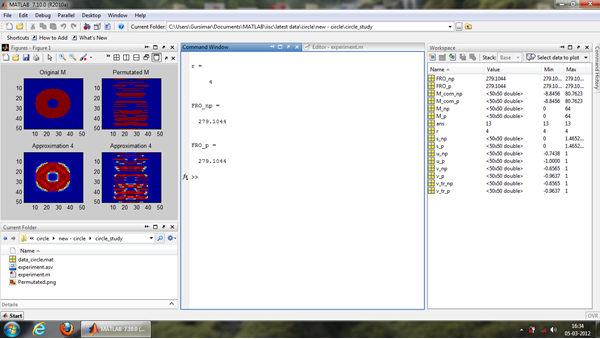
\includegraphics[ height = 70mm,width =115mm]{myfig7.png}
	\end{center}
\end{frame}

\begin{frame}{Rectangular matrix}
	\begin{center}
		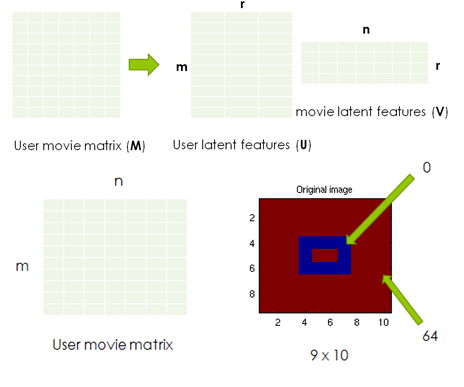
\includegraphics[ height = 70mm,width =115mm]{myfig8.png}
	\end{center}
\end{frame}

\begin{frame}{Rectangular matrix - Initial matrix}
	\begin{center}
		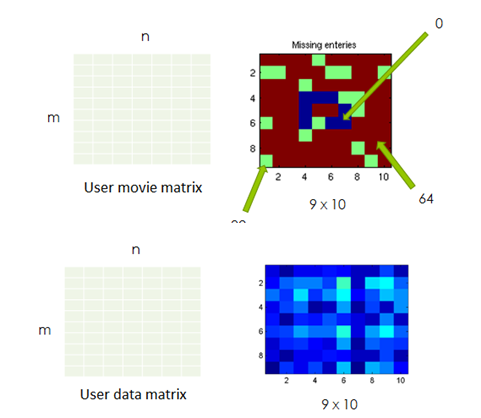
\includegraphics[ height = 70mm,width =115mm]{myfig9.png}
	\end{center}
\end{frame}

\begin{frame}{Rectangular matrix - Recovery}
	\begin{center}
		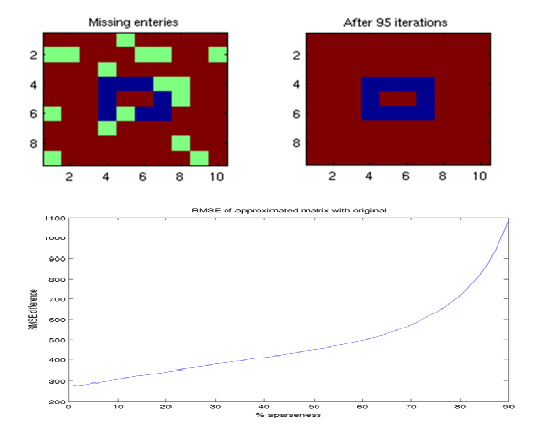
\includegraphics[ height = 70mm,width =115mm]{myfig10.png}
	\end{center}
\end{frame}

\begin{frame}{Rectangular matrix - Permutation}
	\begin{center}
		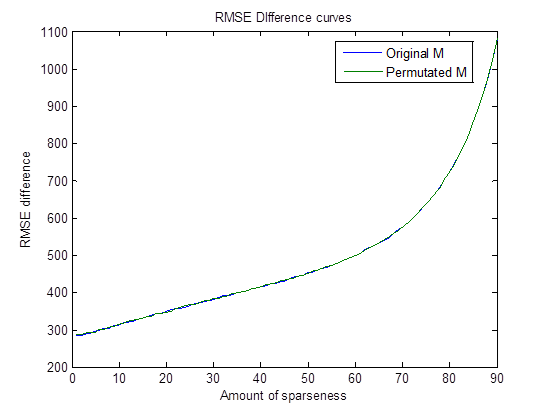
\includegraphics[ height = 70mm,width =115mm]{myfig11.png}
	\end{center}
\end{frame}

\begin{frame}{Rectangular matrix - Comaprison with r>R}
	\begin{center}
		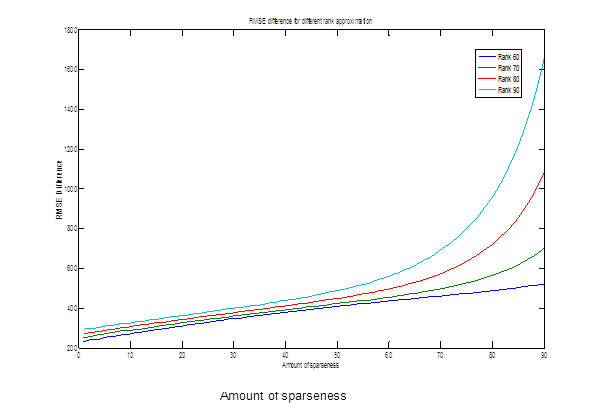
\includegraphics[ height = 70mm,width =115mm]{myfig12.png}
	\end{center}
\end{frame}

\begin{frame}{Rectangular matrix - Circle}
	\begin{center}
		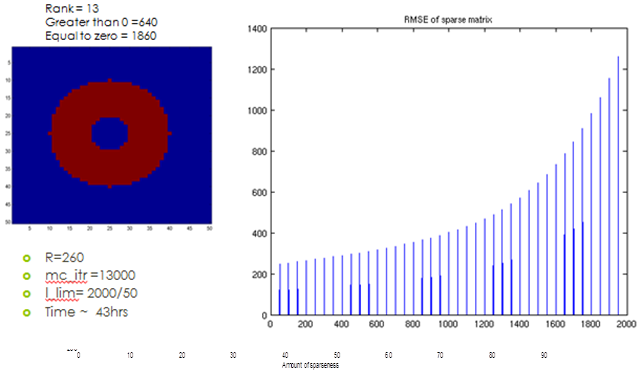
\includegraphics[ height = 70mm,width =115mm]{myfig13.png}
	\end{center}
\end{frame}

\begin{frame}{Testing - distribution testing}
	\begin{center}
		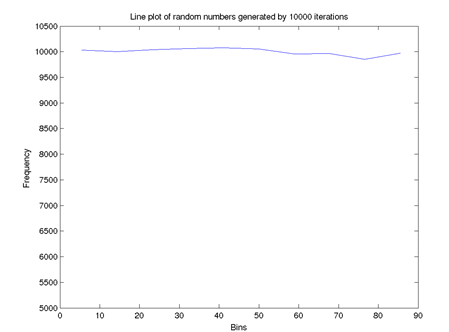
\includegraphics[ height = 70mm,width =115mm]{myfig14.png}
	\end{center}
\end{frame}

\begin{frame}{Testing - Time vs rank}
	\begin{center}
		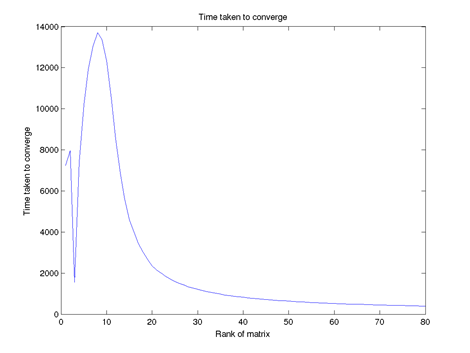
\includegraphics[ height = 70mm,width =115mm]{myfig15.png}
	\end{center}
\end{frame}






\begin{frame}{Applications}
	\begin{itemize}
		\item High dimentionality, but low rank structure.
		\begin{enumerate}
			\item Netflix matrix
			\item Triangulation with sensor net.
			\item Quantum state tomography
			\item Machine learning
			\item Corrupted videos
		\end{enumerate}
		\vspace {3mm}
		\item Robost PCA
		\begin{enumerate}
			\item Recovering foreground from background
			\item Removing shadows from face images.
			\item Batch face alignment 
		\end{enumerate}
		\vspace {3mm}
		\item Transform invariant low rank textures.
		\vspace {3mm}
		\item 3D reconstruction
		\vspace {3mm}
		\item Latent semantic analysis
	\end{itemize}
\end{frame}

% INCLUDE APPLICATIONS IN DETAIL WITH PHOTOGRAPHS...

\end {document}


% understand coupon collector's problem
% try to get some geometric figures of coherence
% 
